\documentclass[12pt]{article}
\usepackage[usenames]{color} %used for font color
\usepackage{amsmath, amssymb, amsthm}
\usepackage{wasysym}
\usepackage[utf8]{inputenc} %useful to type directly diacritic characters
\usepackage{graphicx}
\usepackage [english]{babel}
\usepackage [autostyle, english = american]{csquotes}
\MakeOuterQuote{"}
\graphicspath{ {./} }
\newcommand{\Z}{\mathbb{Z}}
\newcommand{\N}{\mathbb{N}}
\newcommand{\R}{\mathbb{R}}
\newcommand{\Q}{\mathbb{Q}}
\newcommand{\prob}{\mathbb{P}}
\newcommand{\degrees}{^{\circ}}


\author{Tianshuang (Ethan) Qiu}
\begin{document}
\title{Math 74, Week 5}
\maketitle


\section{Mon Lec, 2a}
Let the statement: "There is at most one parallel line to a given line $l$ through a given point $P$." be statement A;
\newline
"If a line intersects one of two parallel lines, both of which are coplanar with the original line, then it also intersects the other." be statement B.
\newline
\begin{figure}[h]
    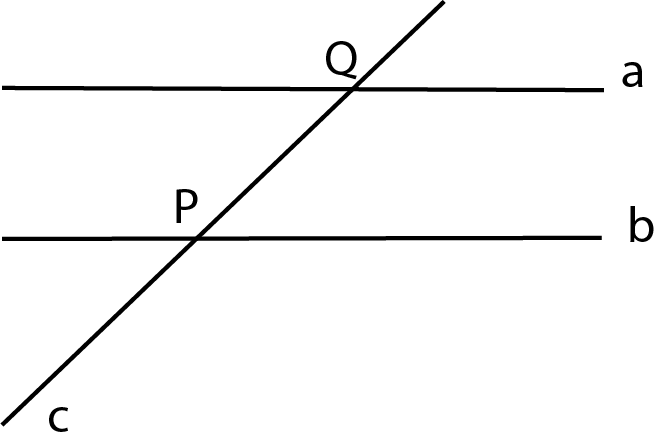
\includegraphics[width = 100mm]{GRAPH1.png}
\end{figure}
\newline
We first prove that $A \implies B$. Let $a \parallel b$, and $c$ intersects $a$ at point $Q$. Assume that statement $B$ is false so $c$ does not intersect $b$. Since it does not intersect and $b$ and $c$ are coplanar, we have $b \parallel c$. $a \parallel b$, and $a, c$ interesect at $Q$. However by $A$ we know that there can be at most one line parallel to $b$ at point $Q$. \lightning. Our assumption is incorrect, $A \implies B$
\newline
Then we show that $B \implies A$. Let $a \parallel b$, and $c$ intersects $b$ at point $P$. Assume that $A$ is incorrect, so we construct $a'$ to also be parallel to $b$. We know that $b$ must intersect $a$ by $B$. We name this point $P$. Then since we have assumed that $a \parallel a'$, our line must also intersect $a'$ at $P$. Consider $\angle SPT, \angle RQT$, and they must be equal because they $a \parallel b$, and corresponding angles are equal when the two lines are parallel. By the same logic we have $\angle SPT = \angle R'QT$.
\newline
Using the transitive property we can get $\angle RQT = \angle R'QT$. However this cannot be true because if the two angles are equal, $a, a'$ overlap and they become the same line. \lightning
\newline
Our assumption is incrroect and $B \implies A$. Therefore $A \iff B$. Q.E.D.

\section{Mon Lec, 3a}
\begin{figure}[h]
    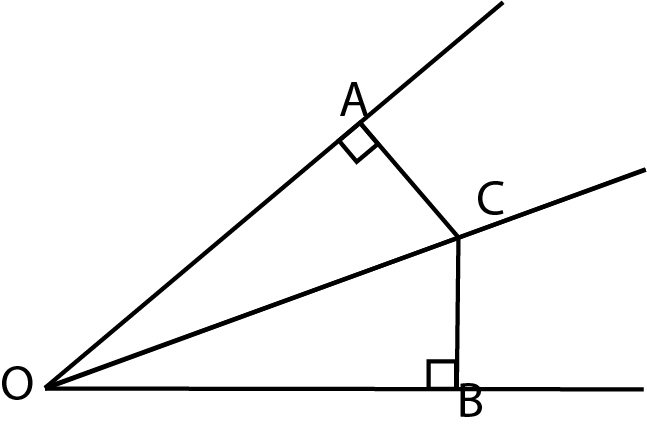
\includegraphics[width = 100mm]{GRAPH2.png}
\end{figure}
\subsection{Bisector $\implies$ equal distance from legs}
Let $OC$ bisect $\angle AOB$, choose $A, B$ such that $CA \perp OA, CB \perp OB$
\newline
Consider $\triangle AOC, BOC$, since $CA \perp OA, CB \perp OB$, we can write the following using the inner sum of triangles:
$$\angle ACO + \angle COA + 90 \degrees = 190 \degrees$$
$$\angle BCO + \angle COB + 90 \degrees = 190 \degrees$$
Since $OC$ bisect $\angle AOB$, we have $\angle COA = \angle COB$, so $\angle ACO = \angle BCO$. Finally, since $\triangle AOC, BOC$ share $OC$, we have $\triangle AOC \cong \triangle BOC$ (ASA congruency). Therefore $CA = CB$. Q.E.D.

\subsection{Equal distance from legs $\implies$ angle bisection}
Let $OC$ be a ray from $O$, choose point C and draw $CA \perp OA, CB \perp OB$. $AC = BC$
\newline
Consider $\triangle AOC, BOC$, since $CA \perp OA, CB \perp OB$, they are both right triangles. Using $AC = BC$, we have $\triangle AOC \cong \triangle BOC$ (HL right triangle congruency). Therefore $\angle COA = \angle COB$.
Q.E.D.
\newpage


\section{Mon Dis, 1b (second bullet)}
$$\prod^{n}_{1}=(1-\frac{1}{n^2})$$
We examine $1-1/k^2$ and factor it into $\frac{k^2-1}{k^2} = \frac{(k+1)(k-1)}{k^2}$. Since k is incrementing by 1 in our series, we can cancel the majority of terms out since it is telescoping. We can expand our series into
$$\frac{1\times 3}{2^2} \times \frac{2 \times 4}{3^2} \times ...\times \frac{(n-1)(n+1)}{n^2}$$
$$= \frac{1}{2} \times \frac{n+1}{n} = \frac{n+1}{2n}$$

\section{Mon Dis, 1d}
(Assuming that )
\subsection{$4^n + 15n -1$}
The largest common divisor for these expressions is $1$.

\subsection{$n^3 - n$}
The largest common divisor for these expressions is $6$.

\subsection{$2^{n+2} + 7n$}
The largest common divisor for these expressions is $5$.
\newpage


\section{Wed Lec, 3a}
Base case: $n = 1, 1 = 1^2$. Base case holds.
\newline
Inductive hypothesis: assume that for some $n \geq 1$, $1+ 3 + 5 + ... + (2n-1) = n^2$.
\newline
Inductive proof: consider $n+1$, $1+ 3 + 5 + ... + (2n-1) + (2n+1)$, using our inductive hypothesis, we can susbsitute everything but the last term: $n^2 + 2n + 1 = (n+1)^2$
\newline
Thus we have proven the inductive step. Q.E.D.

\section{Wed Lec, 3c}
Base case: $n = 1, 1/(4 \times 1^2 - 1) = 1/3 = 1/(2 \times 1 + 1)$. Base case holds.
\newline
Inductive hypothesis: assume that for some $n \geq 1$, $\frac{1}{4 \times 1^2 - 1} + \frac{1}{4 \times 2^2 - 1} + ... + \frac{1}{4 \times n^2 - 1} = \frac{n}{2n+1}$.
\newline
Inductive proof: consider $n+1$, $$\frac{1}{4 \times 1^2 - 1} + \frac{1}{4 \times 2^2 - 1} + ... + \frac{1}{4 \times n^2 - 1} + \frac{1}{4 \times (n+1)^2 - 1}$$
Using our inductive hypothesis, we can susbsitute everything but the last term: $$\frac{n}{2n+1} + \frac{1}{4(n+1)^2 - 1} = \frac{n (4(n+1)^2-1)}{(2n+1)(4(n+1)^2-1)} + \frac{2n+1}{(2n+1)(4(n+1)^2 - 1)}$$
$$=\frac{n(4n^2+3+8n) + 2n +1}{(2n+1)(4n^2+3+8n)} = \frac{4n^3+3n+8n^2+2n+1}{8n^3+6n+16n^2+4n^2+3+8n}=\frac{4n^3+8n^2+5n+1}{8n^3+20n^2+14n+3}$$
We apply long division by $2n+3$ to the denominator.
$$\frac{8n^3+20n^2+14n+3}{2n+3} = 4n^2 + 4n + 1$$
Now we apply long division by $n+1$ to the numerator.
$$\frac{4n^3+8n^2+5n+1}{n+1} =  4n^2 + 4n + 1$$
Therefore we can factor the expression into
$$\frac{(n+1)(4n^2 + 4n + 1)}{(2n+3)(4n^2 + 4n + 1)} = \frac{n+1}{2n+3}$$
\newline
Thus we have proven the inductive step. Q.E.D.

\section{Wed Lec, 6b}
We claim that
\end{document}
